La relación de rechazo de la fuente de alimentación da una medida del rechazo del ruido proveniente de la fuente de alimentación que puede proveer el circuito para distintas frecuencias. En la simulación, se anexó una fuente alterna en serie con cada fuente de alimentación y se pasivó la señal de entrada. Se realizó un barrido en frecuencia con una amplitud \SI{1}{\volt}, obteniendose diversas amplitudes en la salida, según se ilustra en la Figura \ref{fig:psrr}.
\begin{figure}[H]
	\centering
	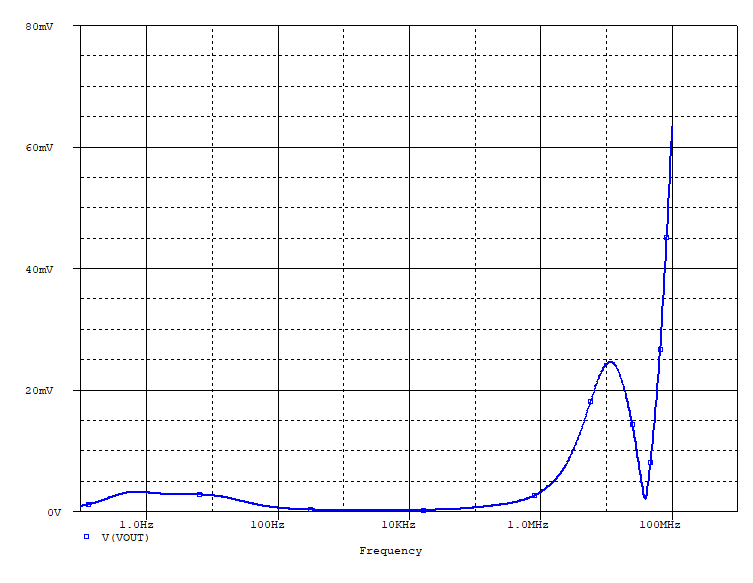
\includegraphics[scale=0.3]{sim_psrr}
	\caption{Rechazo de Ruido de la Fuente.}
	\label{fig:psrr}
\end{figure}

$$ \mathrm{PSRR} [\%]= \frac{v_o}{v_i} = \frac{\SI{2}{\milli\volt}}{\SI{1}{\volt}} = \num{0,002} \%$$
$$ \mathrm{PSRR} [\SI{}{\decibel}] = 20 \cdot \log \left( \frac{\SI{2}{\milli\volt}}{\SI{1}{\volt}} \right) = \SI{-54}{\decibel} $$